
\chapter[Approach]{Approach}
\graphicspath{ {images/approach} }

Comprehending the evolution of a software system is a complex activity, mainly because of the sheer amount of data and its complexity. 
The term "software evolution" was coined for the first time by Lehman in 1985 in a set of laws. \cite{Lehman1985}
He stated that the complexity of a system is destinated to increase over time, as the system always needs to be adapted to its evolutionary environments. 
To be managed, software systems need to be comprehended by developers, and this activity can be simplified with software visualization. 

Over the last ten years, developers have stored their codebase on git repositories. 
For this reason, we focused our attention on systems versioned with this protocol.

Git is a versioning control system that tracks all the changes made to every system file. 
Internally git holds all the information that we need to reconstruct the history of a repository. 

In this chapter, we present our approach for visualizing a software system using a visual and auditive depiction of the evolution of a system. 
To fulfill this purpose, we have chosen to leverage the phenomenon of Synesthesia, the production of a sense impression relating to one sense by stimulation of another sense.
Moreover, we also present how we reconstruct and model the history of a repository. 
\bigbreak
Our approach is composed of three parts: \begin{itemize}
\item in the first part, we model the evolution of a system; 
\item in the second part, we present two ways to visualize the system 
\item in the last part, we show how music can be used to communicate evolutionary information. 
\end{itemize}


\section{Evolution Model}
\label{s:EvolutionModel}

\begin{figure}[H]
    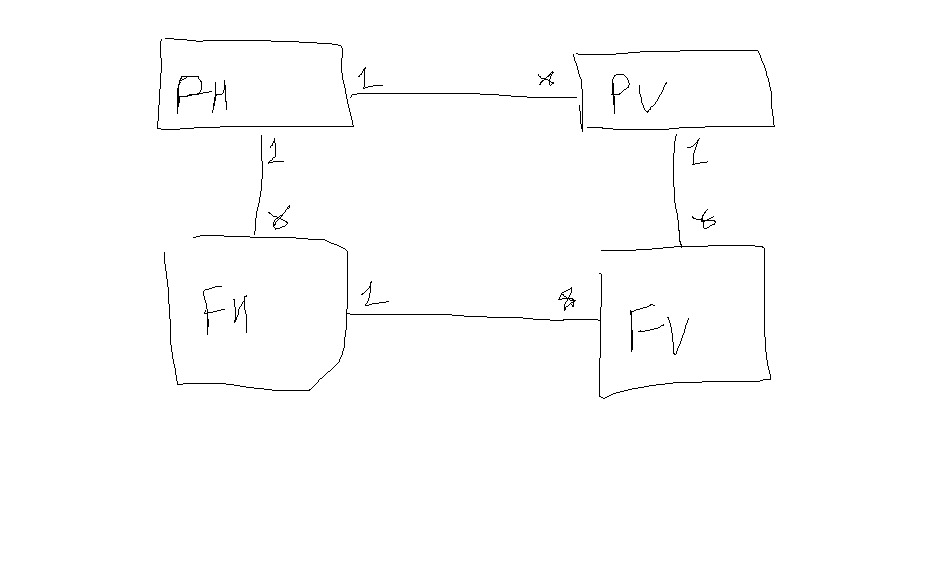
\includegraphics[width=0.6\textwidth]{EvolutionaryModel.jpg}
    \caption{Evolutionary Model}
    \label{fig:EvolutionaryModel1}
\end{figure}

To model the evolution of software systems, we developed the model, 
showed in figure \ref{fig:EvolutionaryModel1}, based on Hismo, a solution presented by Tudor Girba \cite{Girba2005}.\\
\\
The need to develop a novel evolutionary model comes from the fact that Hismo was designed to work with another versioning system: Subversion (SVN). 
There are several differences between SVN and git. In terms of design, the most important is how they keep track of changes. 
SVN works with the concept of "snapshot" while git works with the concept of"commits." 
In SVN, when a file has been changed, a new revision of the whole system is created, and consequently, the number of revisions is incremented. 
In contrast, in git, only the modified files would get committed, and thus we don't have every time a new snapshot of the system. 
Therefore, we took Hismo as the starting point of our model and we adapted it to make it work with the git protocol. 
Initially, the model was based on three concepts:
\begin{itemize}
    \item Snapshot. A representation of the entity whose evolution is studied.
    \item Version. An entity that adds the notion of time to a Snapshot by relating it to History. 
    \item History. An entity that holds a set of Versions.
\end{itemize}
\bigbreak
Git does not have the concept of Snapshot, so we replaced it with a novel concept: FileVersion. 
A FileVersion is essentially the version of a file at a particular point in time. 
It has the same fashion as a Snapshot. Still, instead of being related to every version of the system, it is related only to the Versions where the file was effectively updated.
Moreover, we made a distinction between File entities and Project entities. So, we mapped the concept of History to FileHistory and the idea of Version to ProjectVersion. 
The entity responsible for holding both of them is called ProjectHistory. 
To summarize, these are the four main concepts of our model: 
\begin{itemize}
    \item \textbf{ProjectHistory}: it represents the history of a repository. It is the holder of two sets: a set of FileHistories and a set of ProjectVersions. 
    \item \textbf{FileHistory}: it represents a file of the repository. We consider each file as an entity of the system. Even if the entity's name or location is changed, our mode will treat it as the same. So, our model is resilient to the renaming and moving activities. Each FileHistory holds a set of FileVersion, each one representing a different version of the entity at another point in time.  
    \item \textbf{ProjectVersion}: it represents a commit or a version of the system. 
    For each changed file inside a commit, the respective ProjectVersion contains a FileVersion representing that change.
    A ProjectVersion also holds contextual information about the commit, such as the timestamp, the hash of the commit, and the message.
    \item \textbf{FileVersion}: it represents the version of an entity at a particular point in time.
    It is responsible for holding all evolutionary information of an entity since it represents an evolutionary step of that entity. 
\end{itemize}
\bigbreak

\subsection*{Historical information retrival}
To build the history of a repository, we need to extract the historical information from git.\\
\bigbreak
To understand better how we approached it, we have to explain how git internally represents the repository history. 
Git works with the concept of branches; each branch can be seen as a different repository timeline.
Usually, developers exploit branches to develop features on them and then merge the developed code with the stable codebase.
They need to create a "merge commit" to do that. 
Each time we create a new git commit, we deploy a new version of the system that records all the changes made to the commits' tracked files. 
Internally, in git, all the commits are stored as nodes of a commit tree. 
The root node represents the repository's first commit since it has no parents. 
All the other nodes instead represent the commits made during the whole lifecycle of the repository. 
Each commit usually has only one parent, representing the previous commit made before that one.
There is one case where a commit might have more than one parent: merges commits.
\bigbreak
Each repository should have a branch containing stable, production-ready code as a convention. Usually, this branch is named "main" or "master". 
In our approach, we aim to analyze the timeline of this stable branch. We start from the root of the commit tree, which represents the initial commit, and then we traverse the whole tree. 
However, we don't consider "merge commits" during this process since they already incorporate commits previously made, and thus they would be considered twice. 
Once we have extracted all the valid commits that reside on the stable branch, we need to take from them all the representative information that we need to represent a ProjetctVersion. \\
\bigbreak
Git can recognize the following actions made on a file:
\begin{itemize}
    \item \textbf{ADD}. A file is sent to the repository.
    \item \textbf{DELETE}. A file has been removed from the repository.
    \item \textbf{MODIFY}. A file has been modified.
    \item \textbf{RENAME}. A file's name has been changed. Whether the file path has been changed, the parent directory path must remain the same. 
    \item \textbf{MOVE}. A file was moved from one location to another, so the file path changed. This action detected whether the filename remained the same. 
\end{itemize}

From a commit, we could also extract additional information such as the name of the file being modified, the parent directory, the number of lines added and removed, the path of the file before and after the changes, and many more.
We used the commit's information to track all the paths of an entity. We can update the entity path when it was renamed or moved to follow it during its lifecycle. \\
\linebreak
When we reconstruct the history of a repository, each FileHistory starts with a FileVersion representing an ADD action. Then, in the middle of the FileVersion set, we can find only three kinds of actions: MODIFY, RENAME, and MOVE. 
An entity might be deleted in some cases, so the last FileVersion held by a FileHistory will represent a DELETE action. 

\begin{figure}
    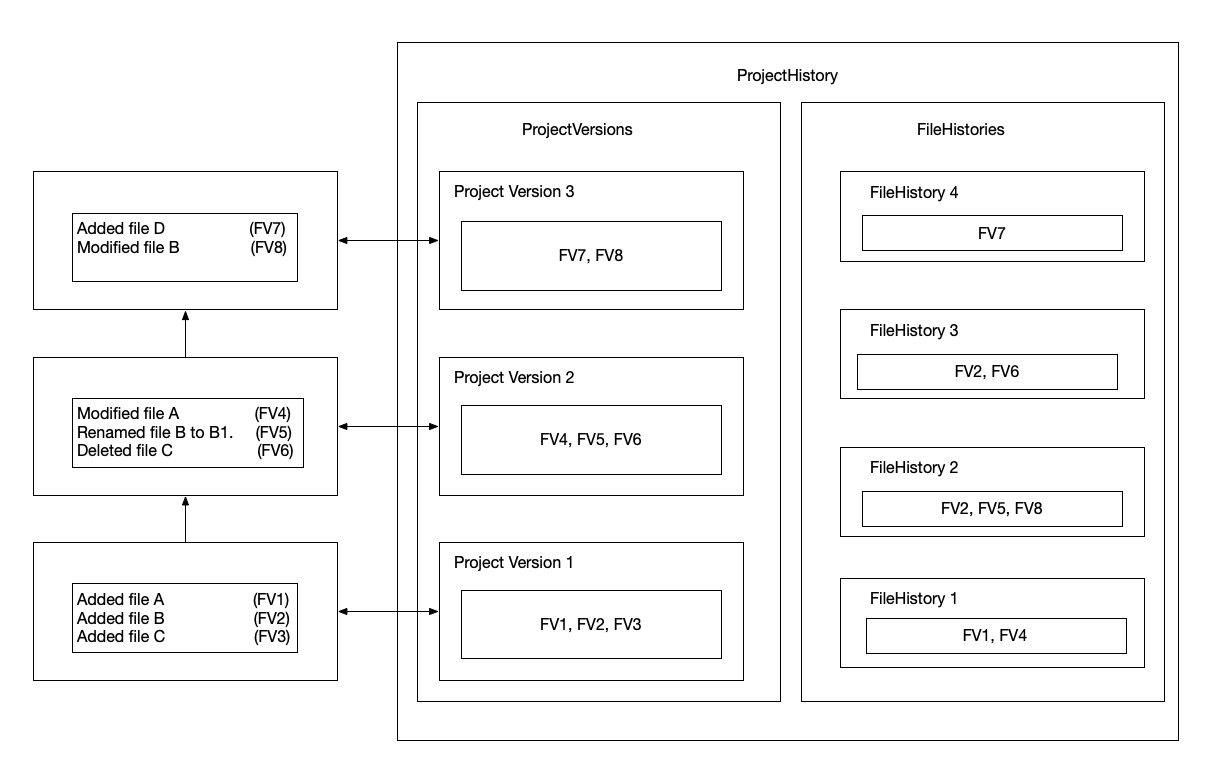
\includegraphics[width=0.6\textwidth]{ApproachExample.png}
    \caption{Rebuilding history example}
    \label{fig:ApproachExample}
\end{figure}

Figure \ref{fig:ApproachExample} shows an example of how history is rebuilt. 
First, we create a ProjectHistory that holds a set of ProjectVersions and a set of FileHistories. 
After that, we start to traverse the repository's commit-tree.
As we can notice, for each commit, we create a new ProjectVersion. It represents a new version of the system in our model. 
Therefore, we inspect the commit's channels and create a new ProjectVersion for each list entry.
With this operation, we can discover if a file has been added to the system because, in that case, the change should represent an ADD operation, and thus we can create a new FileHistory. 
At version 1, three new files were added to the repository (A, B, C), and, as we can see, three new FileHistories were created.
Each change was mapped to a FileVersion (FV) and consequently added to the respective FileHistory and ProjectVersion. 
We did the same thing for ProjectVersion 2 and 3. 

\label{s:partialHistoricalRepr}
\subsection*{Partial historical representation}
One of the goals that we had when we developed this approach was the possibility of analyzing a large repository in an acceptable amount of time. 
In other words, our approach needs to be scalable.
GitHub host the code of some notorious open-source systems, such as LibreOffice, Elastisearch, and Linux.
They all have more than 500,000 commits in each, and thus, we cannot aim to reconstruct their histories with a single analyzer; it will take too much time.  
To prove that, just consider the worse case: Linux. 
When this thesis was redacted, the repository of Linux had 1,090,563 commits. 
To move from one commit to another, we could assume that git needs one second. 
As a result, just to navigate through the whole history of Linux, we would need 11 days.
Moreover, in this simple estimation, we are omitting the vast amount of time that the analyzer needs to extract metrics from every single file on each version. 

We present a scalable approach based on the concept of "partial history" 
A partial history is an entity that holds information about a specific range of time of the ProjectHistory. 
It can be seen as a subset of a ProjetHistory. 
We can split the repository's history into multiple parts, each represented by a partial record. Then when all the analyses are completed, we merge them to reconstruct the whole story of the repository.


\begin{figure}
    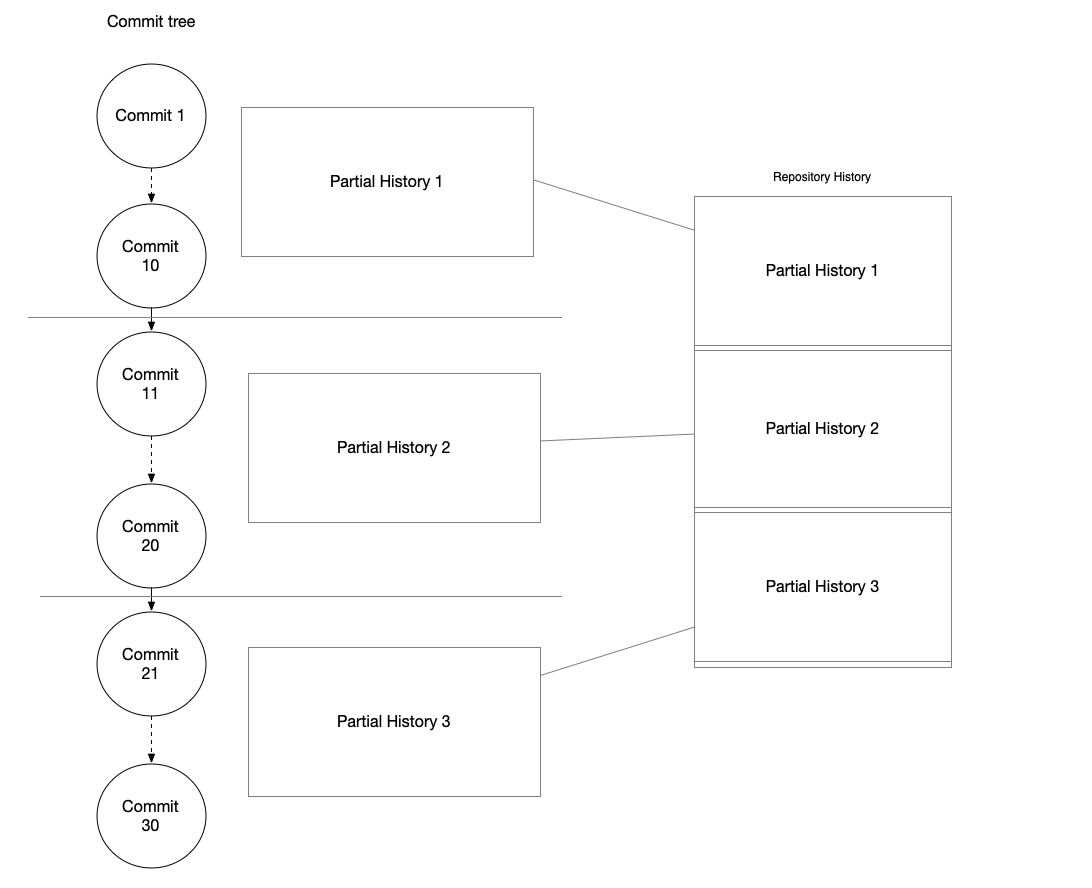
\includegraphics[width=0.6\textwidth]{PartialHistory.png}
    \caption{Partial history example}
    \label{fig:PartialHistory}
\end{figure}

Figure \ref{fig:PartialHistory} shows an example of PartialHistory representation. 
We split the commit tree into multiple chunks, and then we ran the analysis on each piece. 
This analysis can be done in parallel since these chunks are independent of each other. 
In the end, the final history will be represented by a merge of all the PartialHistories. \\
\\
Nonetheless, we can build PartialHistories in parallel; we cannot do the same for the final History. 
The final merge needs to be done sequentially. The sequence needs to follow the order of the commit tree. 
In figure \ref{fig:PartialHistory}, for example
PartialHistory1 represents the history from commit 1 to commit 10, 
PartialHistory2 represents the history from commit 11 to commit 20, and finally 
PartialHistory3 represents the history from commit 21 to commit 30.
Therefore, the commit order is respected if we merge them in this order: 1, 2, 3. 
\\
The result of a single analysis and a parallel analysis must be identical. 
To ensure that, we need to pay attention to the merge operations of our analysis.
When we merge the history of a repository with a partial history, we need to preserve the characteristics of our model. 
In particular, if FileHistory is already present in our history, we don't have to duplicate it, but instead, we need to update it. 

\label{s:evolutionaryMetrics}
\subsection*{Evolutionary metrics}
Every version of the system holds a set of files. 
As we said, each file is represented by a FileVersion, which is part of a FileHistory. 
To understand all the differences between FileVersions of a FileHistory,
we decided to collect metrics to represent the state of a file in a version.\\
\\
Since we aim to have a language-agnostic approach, we have selected only language-agnostic metrics. 
We have defined a taxonomy to classify and categorize all the files present in a system. 
Each category is then mapped to a set of metrics. Moreover, metrics can be inherited by parent categories. \\
\\


\begin{figure}
    \center
    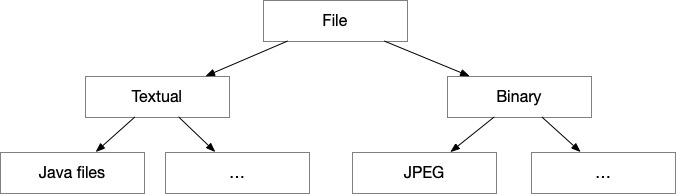
\includegraphics[width=0.6\textwidth]{Taxonomy.jpg}
    \caption{Taxonomy}
    \label{fig:taxonomy}
\end{figure}

We mapped in the following way.

\begin{table}[]
    \begin{tabular}{ll}
    File    & SIZE      \\
    Textual & LOC, LinesAdded, LinesRemoved \\
    Binary  &           \\
    Java    & SLOC
    \end{tabular}
    \caption[]{aaaa}
\end{table}

So, for each file, we compute the metric SIZE, and then, based on the type of the file, if it is a textual file, we also calculate the Lines Of Code (LOC) and the number of lines added and removed. 
In addition, if a file is also a Java file, we compute the Source Lines of Code (SLOC). \\
\\
Our approach can be extended in multiple ways. 
For example, we can define some object-oriented metrics defined only for a particular kind of file, or also, we can introduce a new category (e.g., Object Oriented or Functional). 

\section{Visualization}
The approach that we have defined can be applied to different contexts. 
We can represent a ProjectHistory with two kinds of visualization: a 2D visualization,
 that uses a matrix and works better with small systems, and it is easier to be implemented,
  and a 3D environment that can exploit human perception as a vector of information. 


\subsection*{2D representation}
This visualization is based on the EvolutionMatrix approach defined by Lanza \cite{Lanza2001}. 

We said that a ProjectHistory is a holder of ProjectVersions and FileHistories. 
A ProjectVersion represents a commit or a version of the system, whereas a FileHistory represents the history of a file. 
The connection between these two entities is a FileVersion that describes the state of a file in a system's version. \\
\bigbreak
We can represent a ProjectHistory through a matrix with the following properties: 
\begin{itemize}
    \item Each column of the matrix represents ProjectVersion, so a version of a commit of the repository. 
    \item Each row of the matrix represents a FileHistory, so the history of a file. 
    \item Each cell of the matrix represents a ProjectVersion, so the state of a file is in a specific version. 
\end{itemize}

Since we built our model on the top of git, we don't track snapshots of a system but only change. 
As a consequence, the difference between our matrix and the one defined by Lanza \cite{Lanza2001} is that we can have holes in the row of an entity.
A FileHistory was not modified in a ProjectVersion; this event will be represented by an empty cell.
This concept was not present in the Evolution Matrix of Lanza because its model worked with SVN, and thus, it worked with the idea of incremental snapshots.  

\begin{figure}
    \center
    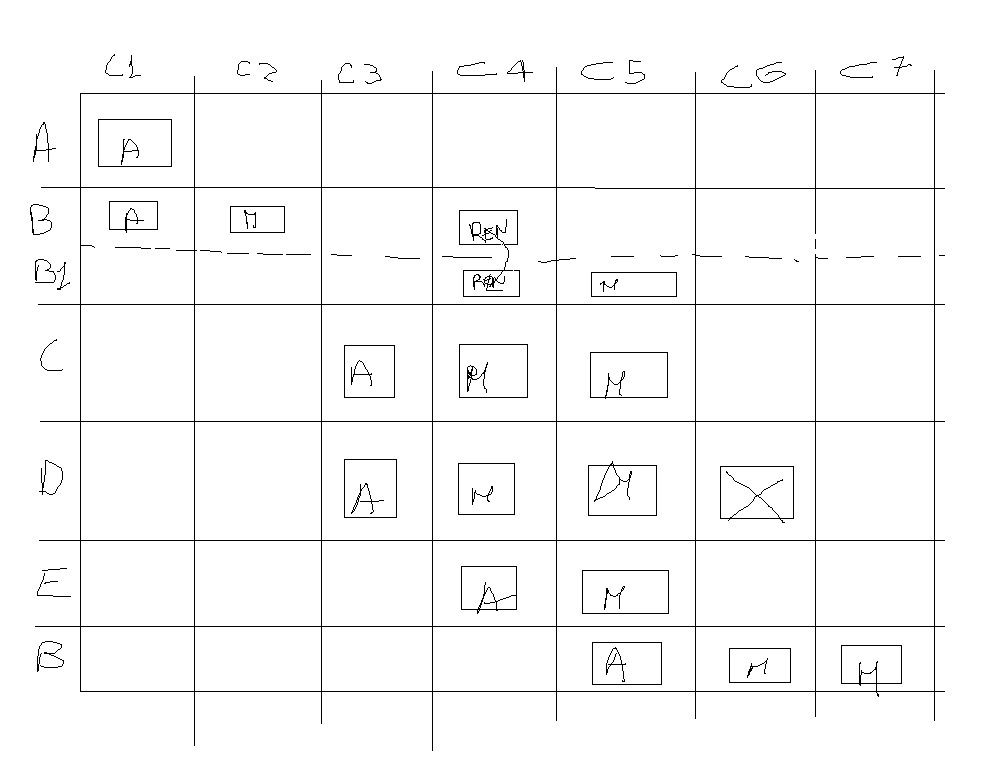
\includegraphics[width=0.6\textwidth]{ApproachMatrix.jpg}
    \caption{Evolution matrix of a repository}
    \label{fig:evolutionMatrixApproach}
\end{figure}
Figure \ref{fig:evolutionMatrixApproach} present a schematic evolution matrix of a repository with seven versions.
As we can see, in the first ProjectVersion, there were added two files, A and B. In the second revision, B was modified, and C and D were added in the third revision.
The fourth revision recorded a rename of B to B1.
It's essential to notice that B and B1 represent the same entity; therefore, the same FileHistory represents them.\\

Based on our aim, we can read this matrix as follows:
 \begin{itemize}
     \item \textbf{by rows}, if we are interested in the history of a particular entity of our system. 
     For example, the FileHistory represented by the first third row in figure \ref{fig:evolutionMatrixApproach} represents the history of the file D. 
     The file D was added in the third ProjectVersion (so the third commit), modified in the fourth and fifth ProjectVersion, and then deleted in the sixth ProjectVersion.
     The figure \ref{fig:evolutionMatrixApproach} is also an excellent example to understand why we cannot rely on the name of the file to identify the entity. 
     We can notice that file B, represented by the second FileHistory, was added on the first version and then renamed on the fourth from B to B1. 
     Then, a new file called B was added in the fifth version. Nonetheless, the name of the files are the same; they must represent two different entities. 
     Even if file B were added in version four, we would have had the same result. 
     \item \textbf{by columns}, if we are interested in which entities were updated on each ProjectVersion. 
    For example, on the first ProjectVersion, we have added the first and the second entity. 
    On the fourth ProjectVersion, we have renamed the second entity, we have modified both the third and the fourth, and finally, we have added the fifth entity.
 \end{itemize}

\begin{figure}
    \center
    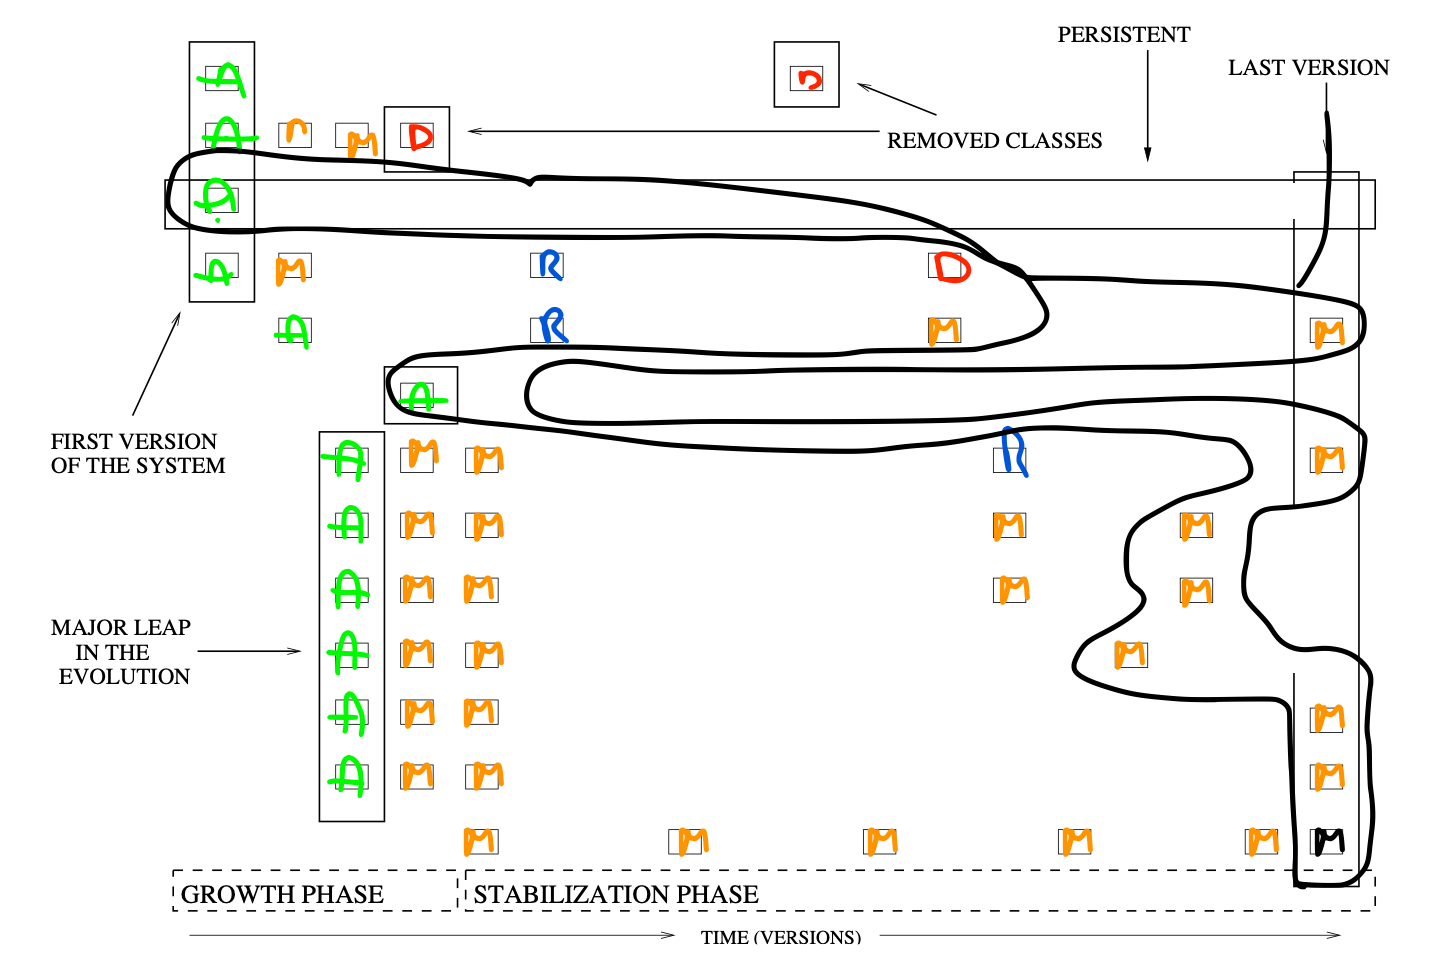
\includegraphics[width=\textwidth]{ApproachMatrix2.png}
    \caption{Evolution matrix of a repository}
    \label{fig:evolutionMatrixApproach2}
\end{figure}

Figure  \ref{fig:evolutionMatrixApproach2} shows an example of how to recover evolution information from the matrix. 
As we have seen, each version does not represent a snapshot of the system.
Instead, it represents only the difference in changes made to the previous version. 
To recover a snapshot of a specific version, we need to consider the last changes made before that particular version.
Under those circumstances, for each FileHistory, we need to go back in time until we find the leftmost change. Of course, if the leftmost difference was deleted, we have to ignore the related FileHistory.
In contrast, if we have to display the evolution of a snapshot, we need to consider only the changes made after that snapshot. 
So, each time we need to display a ProjectVersion, we have to take all its FileVersions and merge them with the current state of the snapshot. 



\subsection*{3D representation}
\label{s:3DRepr}

Software systems are hard to understand due to the complexity and the sheer size of the data to be analyzed.
Our 3D representation aims to make the analysis of a system easier for engineers by exploiting the human senses.
This is why we have chosen to leverage the phenomenon of Synesthesia.
The phenomenon of synesthesia occurs when stimulation of a sense or a cognitive pathway leads to the involuntary stimulation of another reason or a cognitive path.
We experience synesthesia when two or more things are perceived as the same. 
For example, synesthetic people might associate the red color with the letter D or the green color with the letter A. 
There are many forms of synesthesia, each one representing a different type of perception, such as visual forms, auditory, tactile, etc.\\
\\
In our approach, we use the following visual aspects to trigger involuntary associations:
\begin{itemize}
    \item \textbf{Color}: we use the color to describe actions made on an entity (ADD, MODIFY, RENAME, MOVE, DELETE). 
    Ideally, when an entity is deleted, it should be removed from the visualization. This decision is up to the user.  
    \item \textbf{Shape}: we use the shape of the entity to describe the category of the entity. 
    We have defined a taxonomy to categorize entities, and these categories are also mapped. 
    For example, a java file could be represented by a cube, whereas a sphere could represent a binary file.
    \item \textbf{Height}: we use the height of the entity to describe the value of a metric. The decision of which metric is up to the user.
\end{itemize}

\subsection*{Layout}
We developed our visualization approach to visualize the evolution of a system incrementally. 
We cannot track hierarchical relationships with a language-agnostic approach, such as classes belonging to a package. 
So, we have adopted a simple representation that takes care of the creation order of entities.
To layout FileHiistories, we use an outward spiral layout, where the center of the spiral is the first entity added to the system. 

\begin{figure}
    \center
    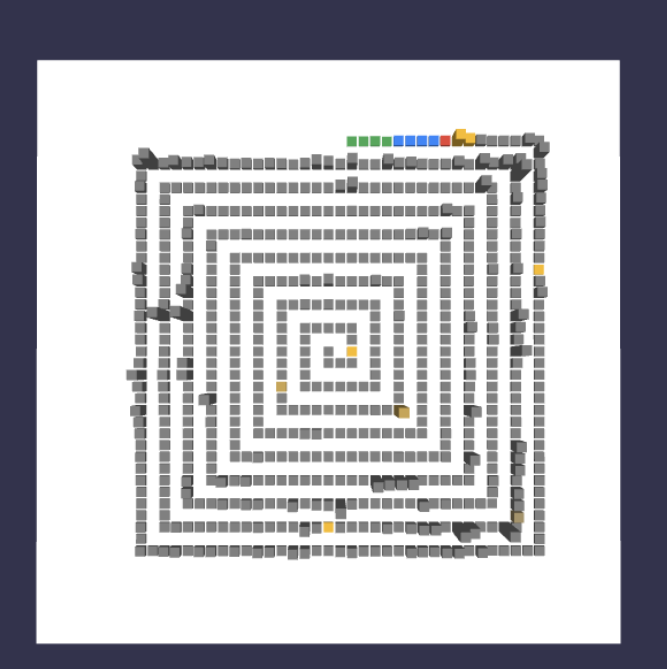
\includegraphics[width=\textwidth]{Layout.png}
    \caption{Spial layout exaple}
    \label{fig:layout}
\end{figure}


\subsection*{Time traversal}

Histories are definer over real human time. Some repositories have been developed for more than ten years. 
Consequently, there are several ways to traverse the history of an entity. 
We can consider the human time or just view the commits made. \\
\bigbreak
The visualization needs to start from the first moment and go forward until the end. 
In our approach, we define two strategies to traverse the history of a repository:
\begin{itemize}
    \item{Strategy 1} We can display \texttt{n} version at the time, so we are traversing the history as it was written. 
    A limitation of this approach is that we lose the concept of time. 
    We cannot have any idea about how much time was passed between the two commits, 
    thus we cannot distinguish active development phases from unactive development phases. 

    \item{Strategy 2} We can group versions by timestamp. 
    So, all the commits made in the same period will be displayed simultaneously. 
    This strategy works very well if we need to comprehend how the system evolved and at which speed in time. 
\end{itemize}

In both our strategies, we might need to aggregate more versions into a single entity: a \textbf{moment}. 
We define a moment as a group of versions that will be displayed simultaneously. 

\begin{figure}[H]
    \begin{center}
        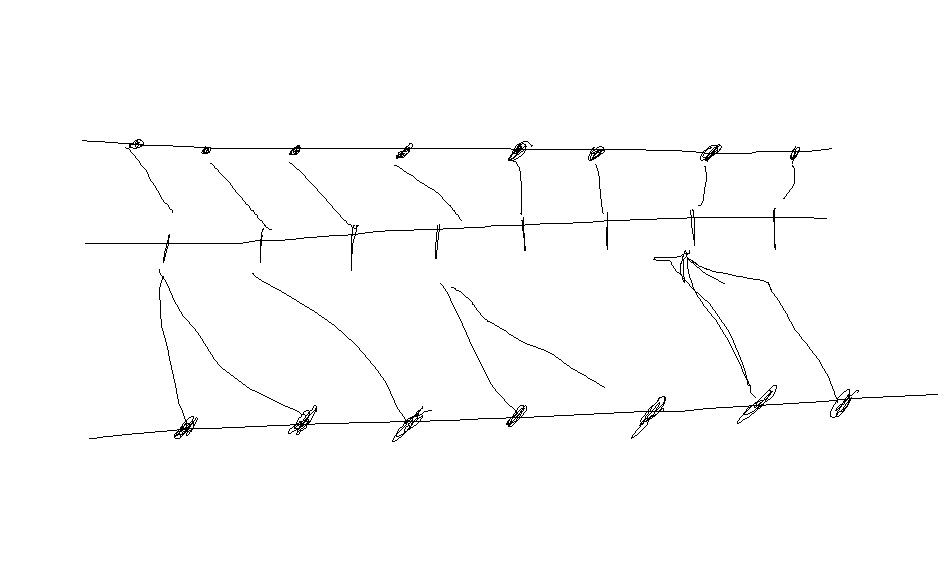
\includegraphics[width=0.9\linewidth]{Moments.jpg} 
        \caption{Example of two different strategies to identity moments. 
        In the first strategy, we mapped one commit with one moment, so the number of moments will equal the number of commits.  
        Alternatively, in the second strategy, we created a moment every day.
        As a result, we have moments with many commits and some without anyone.
        With this strategy, the number of moments will be the same as the number of days between the first and the last commit. 
        }
        \label{fig:moment}
    \end{center}
\end{figure}

Figure \ref{fig:moment} highlights the difference between the two strategies mentioned above. 


\subsection*{Color}
\begin{wrapfigure}{r}{0.3\textwidth}
    \begin{center}
        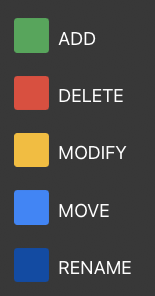
\includegraphics[width=0.7\linewidth]{ColorAssociation.png} 
        \caption{Color association}
        \label{fig:ColorAssociation}
    \end{center}
\end{wrapfigure}

The entity's color should recall the last action made on that entity. To achieve this purpose, we used the color association described in figure \ref{fig:ColorAssociation}.
Nonetheless, each person has their perception of colors. Thus, we can not assume that this color will work similarly for all people.
To remedy this issue, users can customize the color palette. \\
\\
We decided to put another piece of information on the color of the entity: the \textbf{aging}. 
We define the aging of an entity as the number of moments since the last modification of that entity happened.
We mapped the age of an entity with the darkness of its color to do that. 
As a result, older entities will be displayed with a darker color. 
This way, users can immediately recognize the last action and the time passed since the entity was modified.


\subsection*{Shape}
We have chosen to play with the entity's shape to distinguish them based on their type. 
Our visualization layout works with an outward spiral that always adds a new entity at the tail. 
If a commit involves lots of entities, it would be helpful to know immediately which kinds of entities are modified. 
For this reason, we mapped the entity's shape to the file type of the entity itself.
Usually, there are many file types in a repository, so we cannot aim to have an exhaustive set of shapes to represent each file type individually. 

\subsection*{Height}
As we said, the height of an entity must represent the value of a chosen metric. 
Entities without the selected metric would not be represented in our approach. 

To extract the value of the height from a metric, we used to map it with a \textbf{mapper}.
A mapper is defined as a function that returns its height given an entity and a metric.\\
\\
This mapping function might be defined in several ways, such as with a linear process whose maximum value is predefined and its minimum value is 0. 
The choice of which strategy should be used is up to the user. 



\section{Auditive model}

We supported our visualization approach with an auditive portrayal of ProjectVersions being displayed. The goal is to transmit information such as the number of version changes, number of additions, and number of deletions, through audio notes. 

We investigated several approaches to map evolutionary metrics to sound; as a result, our approach uses the following audio concepts:
\begin{itemize}
	\item BPM: Beats Per Minute or tempo sets the rhythm of a song. 
	\item Note's pitch: the quality that makes it possible to judge sounds as "higher" and "lower" in a sense associated with musical melodies.
	\item Synthesizer: a producer of audio signals. 
\end{itemize}

As we said, our visualization works over the concept of moments. We mapped each moment to a sound that is generated procedurally. 
Each sound is composed of three different synthesizers. We used them to distinguish between the three pieces of information that we want to provide: number of version changes, number of additions, and number of deletions. Moreover, the note reproduced by each synthesizer depends on the magnitude of the metric. For example, if we compose the sound of a moment that holds lots of additions, the note played by the synthesizer that represents additions will be high. In contrast, a moment with few additions will be mapped to a note with a low pitch. Finally, the tempo depends on the number of changes in our approach. So a moment with lots of changes will sound more fierce than a moment with few changes. 













